\section{Intro}
\label{sec:intro}
\textit{"You are going to develop a travel-planning system in which you will need to implement a method for computing the cheapest route between destinations. \\
Data about the destinations and possible routes between them are placed in a file (to be found on black board next to the assignment) where each line contains a destination followed by the cities to which you can travel and the associated cost. \\
Notice that even though there is a route from A to B, there might not be one from B to A."}

\section{To be hand in}
\todo[inline]{A short description of which methods and data structures you have chosen.}
\todo[inline]{At least 3 examples where you use your algorithms to investigate the existence of routes and plan
the cheapest one.}
\todo[inline]{Benchmarks for how long it takes to plan a route.
Code needs to be delivered in an appendix.}


\section{Solution}
\subsection{Question \#1}
\todo[inline]{Some kind of pseudo code}
A routine for loading in the file and appropriate data structures for representing the data is shown in appendices \ref{app:FileHandle} and \ref{app:Vertex}.\\
We are using a Hash-map where the from cities are associated with accesable towns and thier egde cost.



\subsection{Question \#2}
\todo[inline]{Some kind of pseudo code}
\todo[inline]{Print from Odense for later use}
A method for determining which cities you can reach from a given start city.


\subsection{Question \#3}
\todo[inline]{Some kind of pseudo code}
\todo[inline]{Why we use the dijkstras algorithm}
We have chosen to use the Dijkstras algorithm for computing the quickest route between two destinations. The properties of Dijkstras algorithm producing a shortest path tree for a graph data structure with non-negative edge path costs. \\

The complexity of the algorithm 


\begin{lstlisting}
function Dijkstra(Graph, source):
    dist[source] := 0                     // Initializations
    for each vertex v in Graph:           
        if v != source
            dist[v] := infinity           // Unknown distance from source to v
            previous[v] := undefined      // Predecessor of v
        end if
        Q.add_with_priority(v,dist[v])
9      end for 
10
11
12     while Q is not empty:                 // The main loop
13         u := Q.extract_min()              // Remove and return best vertex
14         mark u as scanned
15         for each neighbor v of u:
16             if v is not yet scanned:
17                 alt = dist[u] + length(u, v) 
18                 if alt < dist[v]
19                     dist[v] := alt
20                     previous[v] := u
21                     Q.decrease_priority(v,alt)
22                 end if
23             end if
24         end for
25     end while
26     return previous[]

\end{lstlisting}



This algorithm is often used in routing and as a subroutine in other graph algorithms.


\section{Examples and Benchmarks}



\subsection{Odense to Aalborg}

\begin{figure}[th!]
\centering
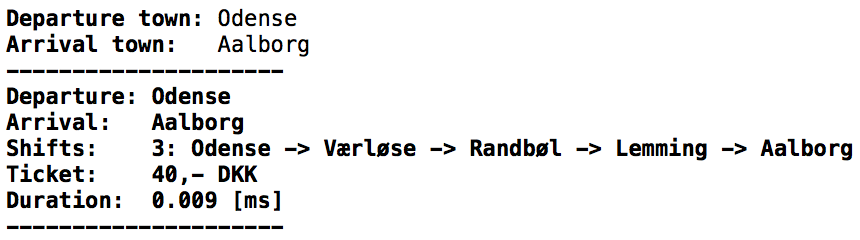
\includegraphics[width=0.7\textwidth]{./graphics/ex1}
\caption{Output from editor: Odense to Aalborg.}
\label{fig:odense_Aalborg}
\end{figure}

	
\subsection{Odense to Holstebro}

\begin{figure}[th!]
\centering
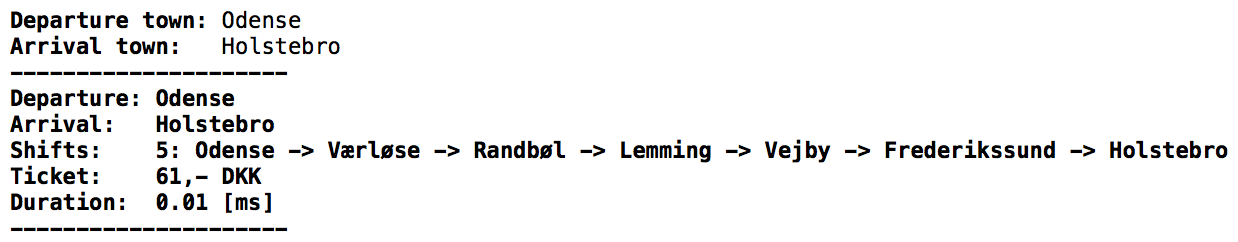
\includegraphics[width=0.7\textwidth]{./graphics/ex2}
\caption{Output from editor: Odense to Holstebro.}
\label{fig:odense_holstebro}
\end{figure}

\subsection{Odense to Humlebæk}

\begin{figure}[th!]
\centering
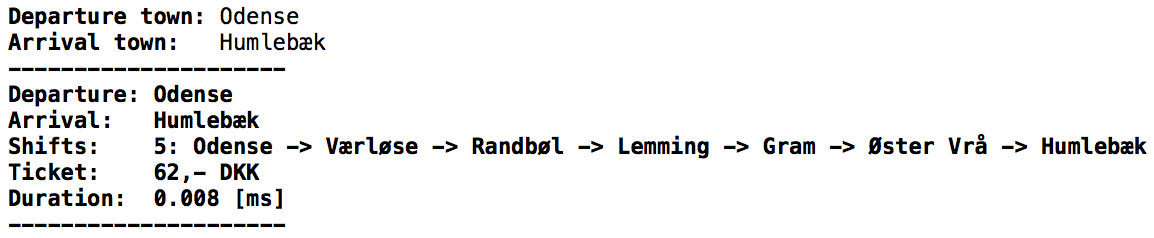
\includegraphics[width=0.7\textwidth]{./graphics/ex3}
\caption{Output from editor: Odense to Humlebæk.}
\label{fig:odense_humlebæk}
\end{figure}






